% This must be in the first 5 lines to tell arXiv to use pdfLaTeX, which is strongly recommended.
\pdfoutput=1
% In particular, the hyperref package requires pdfLaTeX in order to break URLs across lines.

\documentclass[11pt]{article}

% Change "review" to "final" to generate the final (sometimes called camera-ready) version.
% Change to "preprint" to generate a non-anonymous version with page numbers.
\usepackage{acl}

% Standard package includes
\usepackage{times}
\usepackage{latexsym}

% For proper rendering and hyphenation of words containing Latin characters (including in bib files)
\usepackage[T1]{fontenc}
% For Vietnamese characters
% \usepackage[T5]{fontenc}
% See https://www.latex-project.org/help/documentation/encguide.pdf for other character sets

% This assumes your files are encoded as UTF8
\usepackage[utf8]{inputenc}

% This is not strictly necessary, and may be commented out,
% but it will improve the layout of the manuscript,
% and will typically save some space.
\usepackage{microtype}

% This is also not strictly necessary, and may be commented out.
% However, it will improve the aesthetics of text in
% the typewriter font.
\usepackage{inconsolata}

%Including images in your LaTeX document requires adding
%additional package(s)
\usepackage{graphicx}

% If the title and author information does not fit in the area allocated, uncomment the following
%
%\setlength\titlebox{<dim>}
%
% and set <dim> to something 5cm or larger.

\title{Instructions for *ACL Proceedings}

% Author information can be set in various styles:
% For several authors from the same institution:
% \author{Author 1 \and ... \and Author n \\
%         Address line \\ ... \\ Address line}
% if the names do not fit well on one line use
%         Author 1 \\ {\bf Author 2} \\ ... \\ {\bf Author n} \\
% For authors from different institutions:
% \author{Author 1 \\ Address line \\  ... \\ Address line
%         \And  ... \And
%         Author n \\ Address line \\ ... \\ Address line}
% To start a separate ``row'' of authors use \AND, as in
% \author{Author 1 \\ Address line \\  ... \\ Address line
%         \AND
%         Author 2 \\ Address line \\ ... \\ Address line \And
%         Author 3 \\ Address line \\ ... \\ Address line}

\author{Isaac Peterson \\
  \texttt{isaac.peterson@usu.edu} \\\And
  Second Author \\
  \texttt{email@domain} \\\And 
  Third Author \\
  \texttt{email@domain} 
  }

%\author{
%  \textbf{First Author\textsuperscript{1}},
%  \textbf{Second Author\textsuperscript{1,2}},
%  \textbf{Third T. Author\textsuperscript{1}},
%  \textbf{Fourth Author\textsuperscript{1}},
%\\
%  \textbf{Fifth Author\textsuperscript{1,2}},
%  \textbf{Sixth Author\textsuperscript{1}},
%  \textbf{Seventh Author\textsuperscript{1}},
%  \textbf{Eighth Author \textsuperscript{1,2,3,4}},
%\\
%  \textbf{Ninth Author\textsuperscript{1}},
%  \textbf{Tenth Author\textsuperscript{1}},
%  \textbf{Eleventh E. Author\textsuperscript{1,2,3,4,5}},
%  \textbf{Twelfth Author\textsuperscript{1}},
%\\
%  \textbf{Thirteenth Author\textsuperscript{3}},
%  \textbf{Fourteenth F. Author\textsuperscript{2,4}},
%  \textbf{Fifteenth Author\textsuperscript{1}},
%  \textbf{Sixteenth Author\textsuperscript{1}},
%\\
%  \textbf{Seventeenth S. Author\textsuperscript{4,5}},
%  \textbf{Eighteenth Author\textsuperscript{3,4}},
%  \textbf{Nineteenth N. Author\textsuperscript{2,5}},
%  \textbf{Twentieth Author\textsuperscript{1}}
%\\
%\\
%  \textsuperscript{1}Affiliation 1,
%  \textsuperscript{2}Affiliation 2,
%  \textsuperscript{3}Affiliation 3,
%  \textsuperscript{4}Affiliation 4,
%  \textsuperscript{5}Affiliation 5
%\\
%  \small{
%    \textbf{Correspondence:} \href{mailto:email@domain}{email@domain}
%  }
%}

\begin{document}
\maketitle
\begin{abstract}
  In this project, we explore the application of reinforcement learning (RL) to train an agent capable of navigating a 2D grid environment and identifying geometric shapes with distinct colors. The agent recieves instruction via natural langauge and then the agent moves one space at a time across the grid, using RL techniques to learn an optimal policy for efficiently locating and identifying shapes such as green triangles and red squares. We define the task as a partially observable Markov decision process (POMDP), where the agent's observations are limited to the grid space it occupies. Our approach involves implementing Reinforcement Learning to teach the agent to maximize rewards by minimizing the time and steps required to find and correctly identify a shape. The results demonstrate how reinforcement learning can be applied to shape recognition and navigation tasks, with potential applications in robotics, search-and-rescue missions, and autonomous systems. If time permits, we want to further explore what modifications need to be made in order to command a fleet of agents to accomplish tasks in an optimal manner.

\end{abstract}

\section{Introduction}
As technologies continue to advance, the integration of robots into every day life is continuing to increase. As humans rely mostly on speech for communication and instruction, it is essential that robots are also developed to understand and decipher language, executing commands via effectively and efficiently. 

There are a myriad of challenges that one confronts when attempting to solve this problem. First and foremost, establishing an interface between the spoken command and correct execution of that command. To properly execute the spoken command, the agent needs to have an accurate understanding of its environment, which in the real world can become extremely complex. Initial attempts were made by utilizing more logic based methods to help the robot understand the task that needs to be solved \cite{Liu2016}. To mitigate the challenges that come with real world interpretation, many researchers defaulted to simulations to instruct agents in a more structured world.

Video games form a natural challenge for agents, with clear tasks to complete in a very structured world. \cite{Chaplot2017} used the environment in the video game DOOM\texttrademark to train their agent to follow natural language instructions, with other researchers using similiary techniques in Minecraft\texttrademark \cite{Tessler2020}, and even developing their own virtual environments for natural language task completion \cite{Anderson2017} \cite{Wang2024}. 

Our goal is to use the simplified environment in Minigrid \cite{MinigridMiniworld23} to explore the process of natural langauge task completion, with more research on the multi-agent natural language task completion problem. Where instead of instructing a single agent to complete a task, we instruct a fleet of agents and explore the challenges that come with the increased number of agents along with solution to address these challenges. 

\section{Related Work}
Most of the work in this project will be based on the work done by \cite{Chaplot2017}. They utilize a combination of large language models and reinforcement learning to help an agent understand specific instructions to navigate in the game environment of doom. Others utlized the world of minecraft to help agents complete tasks, with less of a focus on instruction and more on generalized learning rather than interpreting language \cite{Oh2017}, \cite{Tessler2020}. Combining the implementation of \cite{Chaplot2017} with the Minigrid environment \cite{MinigridMiniworld23}, \cite{chevalier2018babyai} we can further explore the challenging problem of robotic instruction with large language models, with the added challenge of addressing multiple agents.

\section{Methods}
\begin{figure*}[!t]
  \centering
  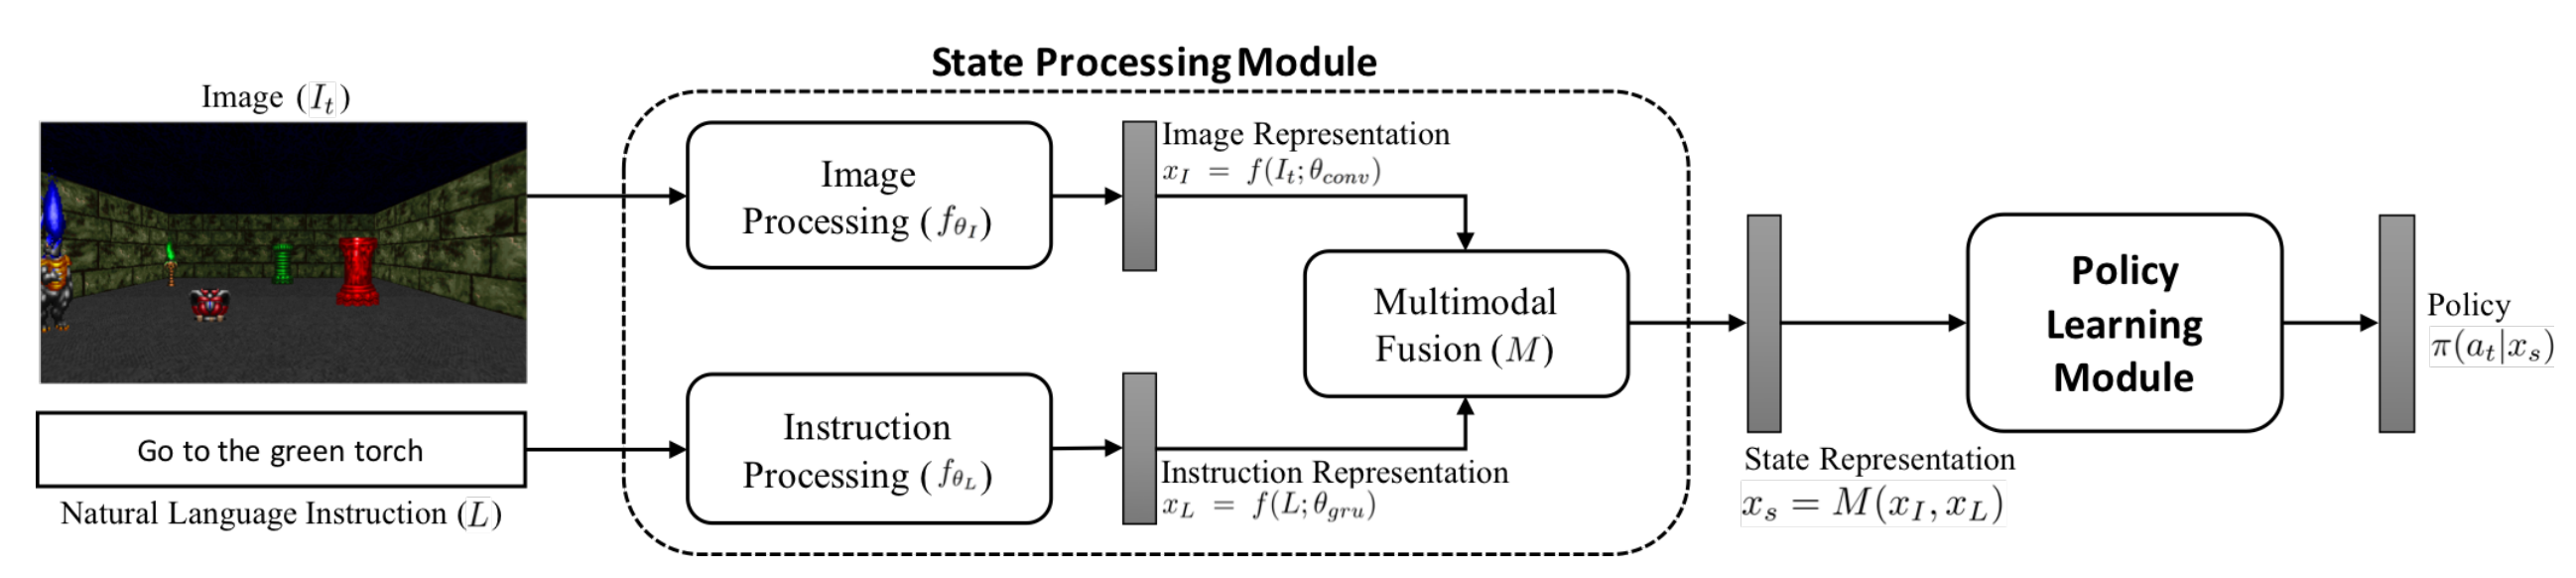
\includegraphics[width=\linewidth]{figs/stateprocessing.png}
  \caption{State processing method as developed by \cite{Chaplot2017}.}
  \label{fig:stateprocess}
\end{figure*}

The Minigrid environment is available on a public repository in github. Which will form the foundation for the work that we will present in this research. Also foundational to our research is the State Processing Module as shown in Figure~\ref{fig:stateprocess}. Our modified state processing module to use the Minigrid environment and handle multiple agents is shown in Figure~\ref{fig:modeloverview}.





\begin{figure*}[!t]
  \centering
  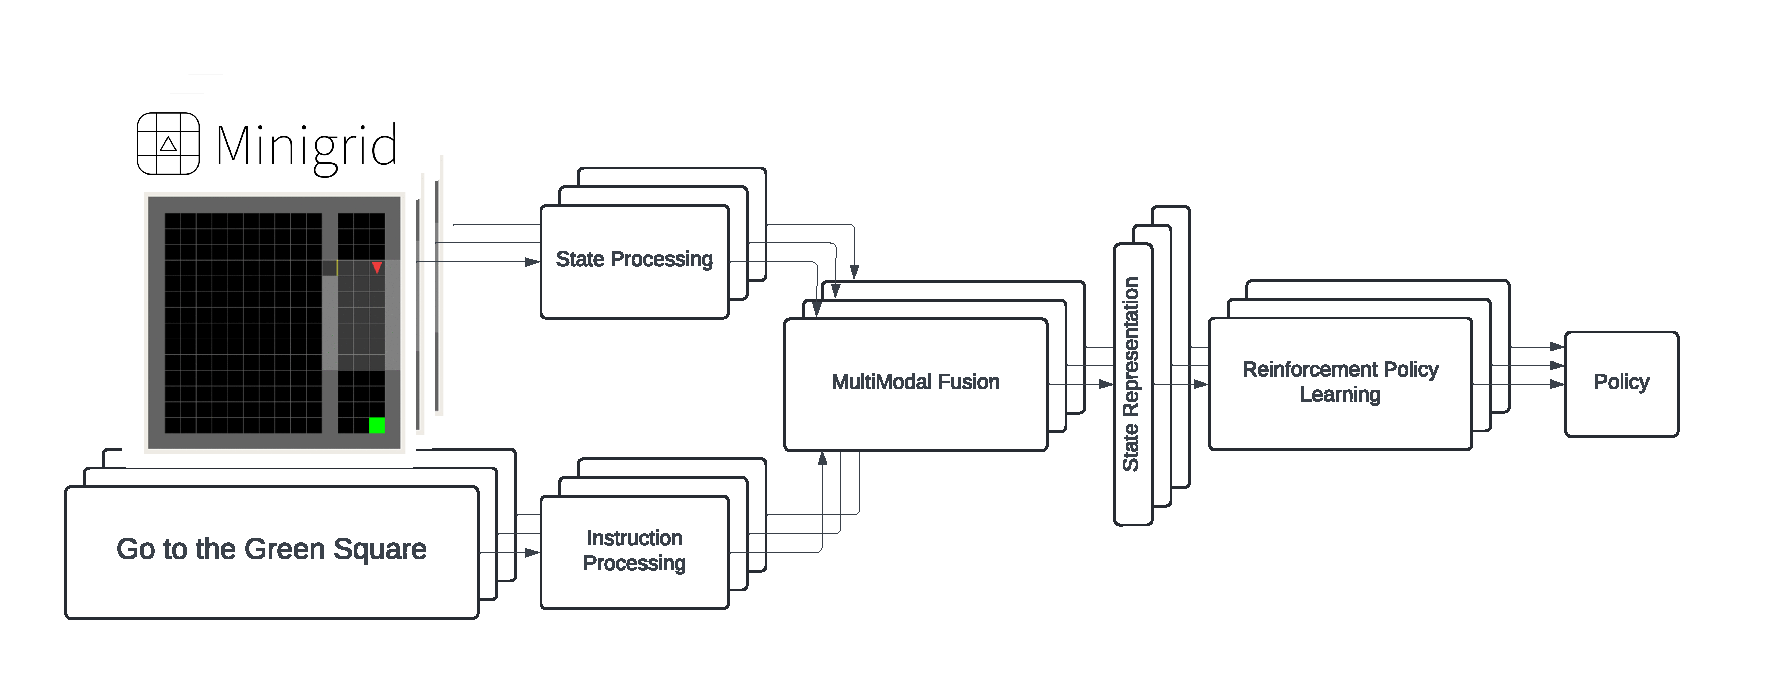
\includegraphics[width=\linewidth]{figs/modeloverviewactual.pdf}
  \caption{Our approach to solving the multi-agent natural language task-solving problem, showing layers for each agent.}
  \label{fig:modeloverview}
\end{figure*}




% \bibliographystyle{plain}

\bibliography{custom}
\end{document}
